\providecommand{\main}{../../../..}
\documentclass[\main/dresen_thesis.tex]{subfiles}
\begin{document}
  \label{sec:colloidalCrystals:layers:gisaxs}
  \begin{figure}[tb]
    \centering
    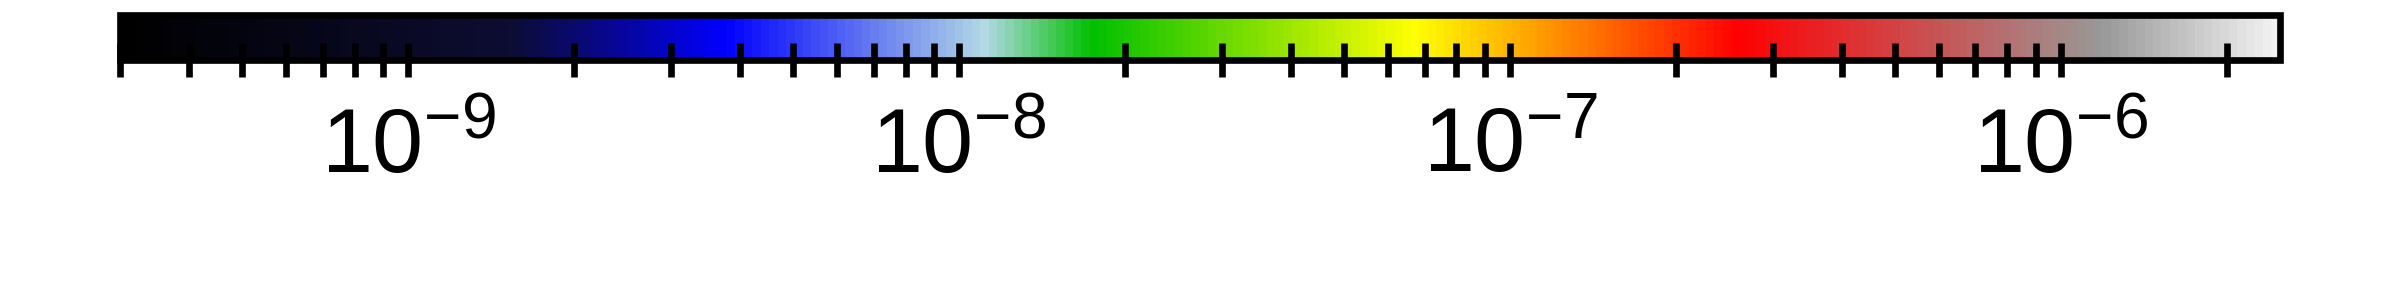
\includegraphics{colloidalCrystals_GISAXS_SVcbar}
    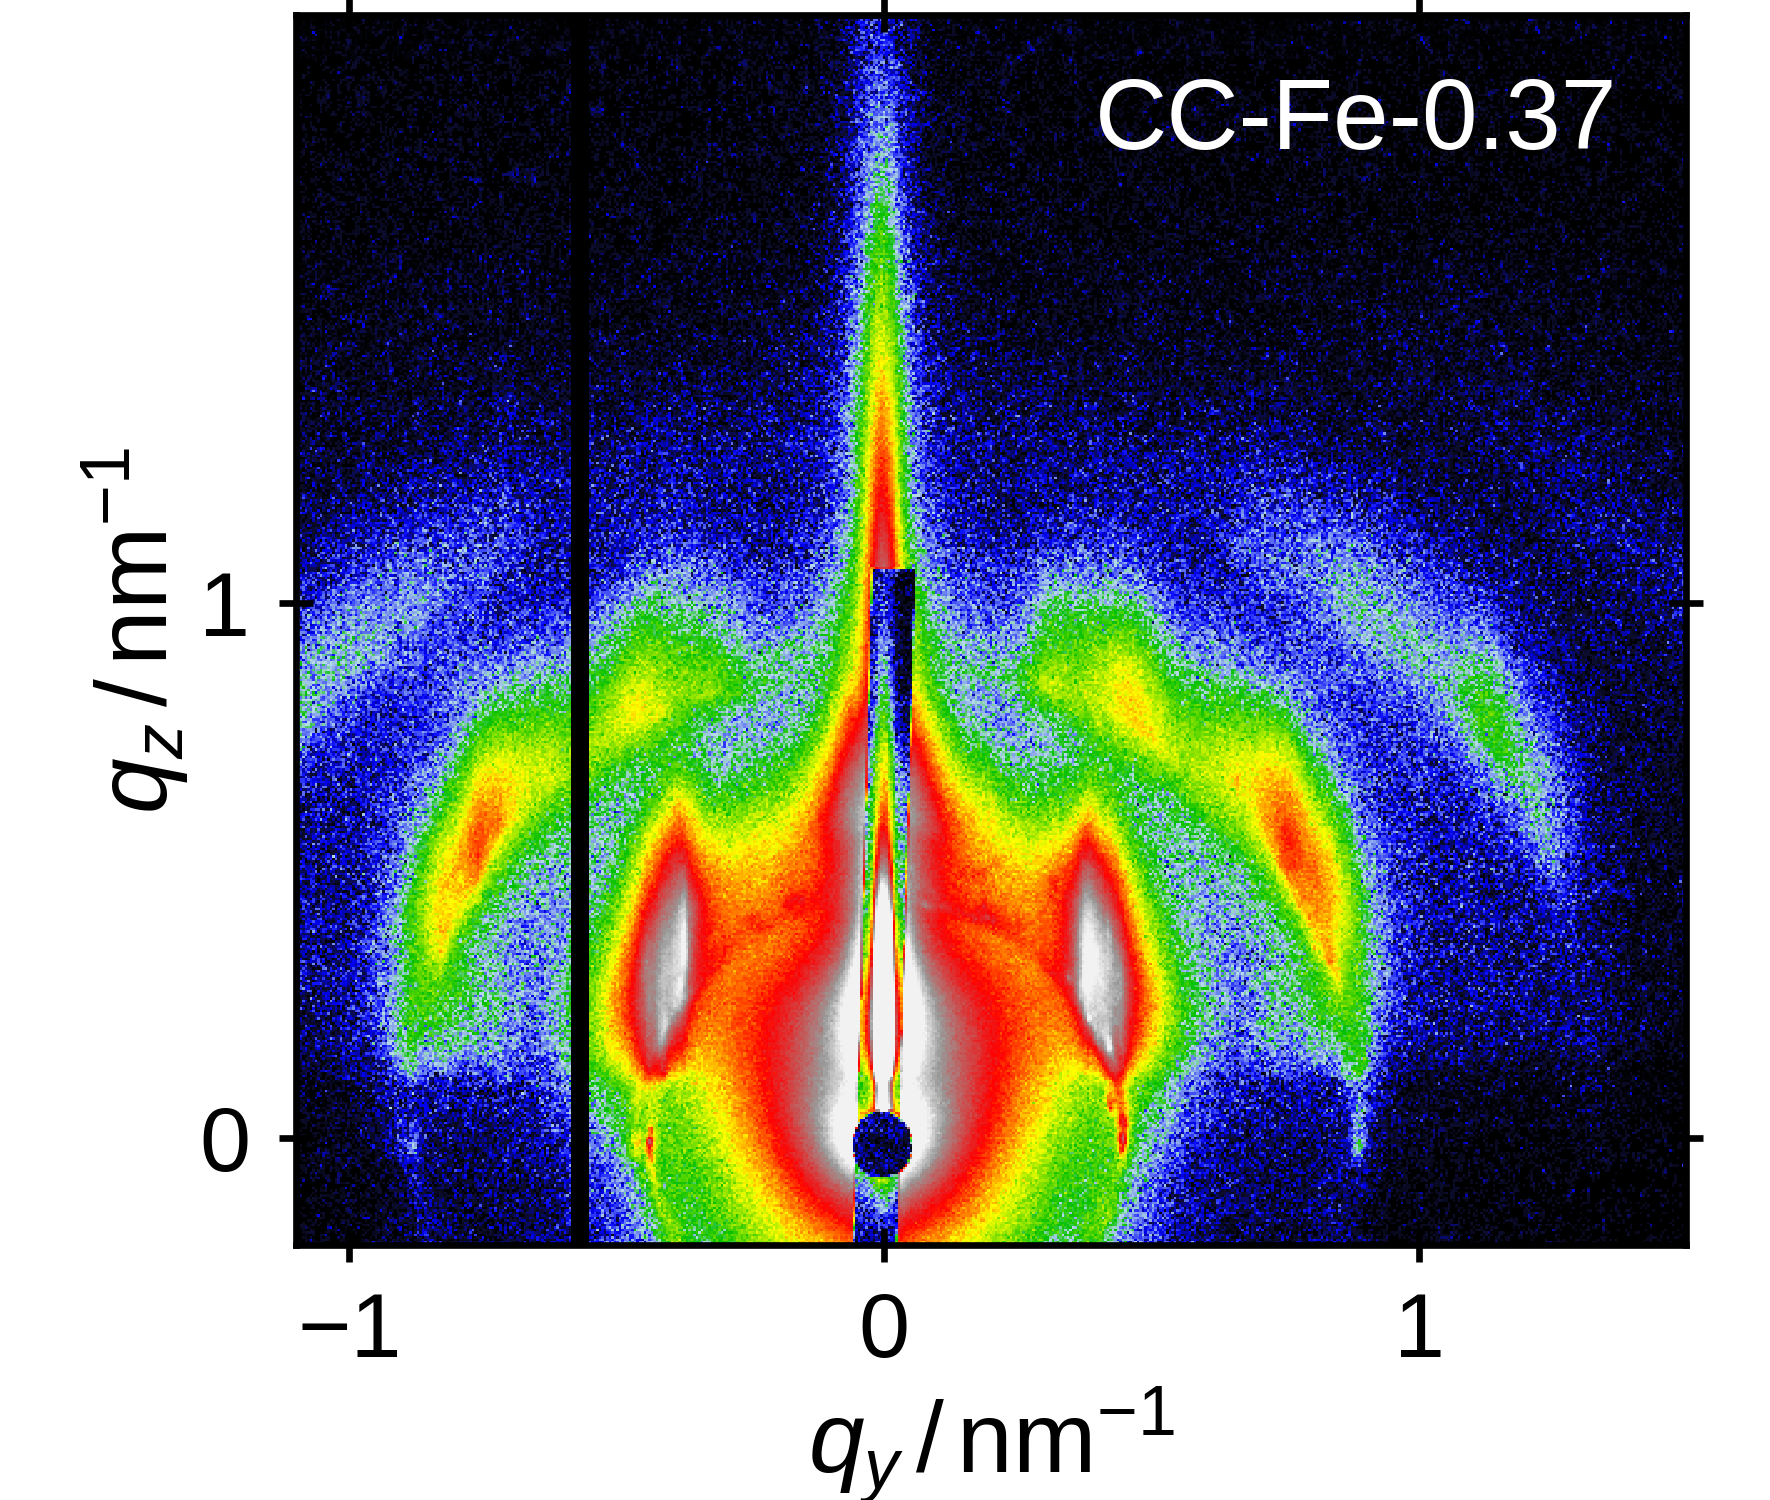
\includegraphics{colloidalCrystals_GISAXS_CC-Fe-0_37_lowerAngle}
    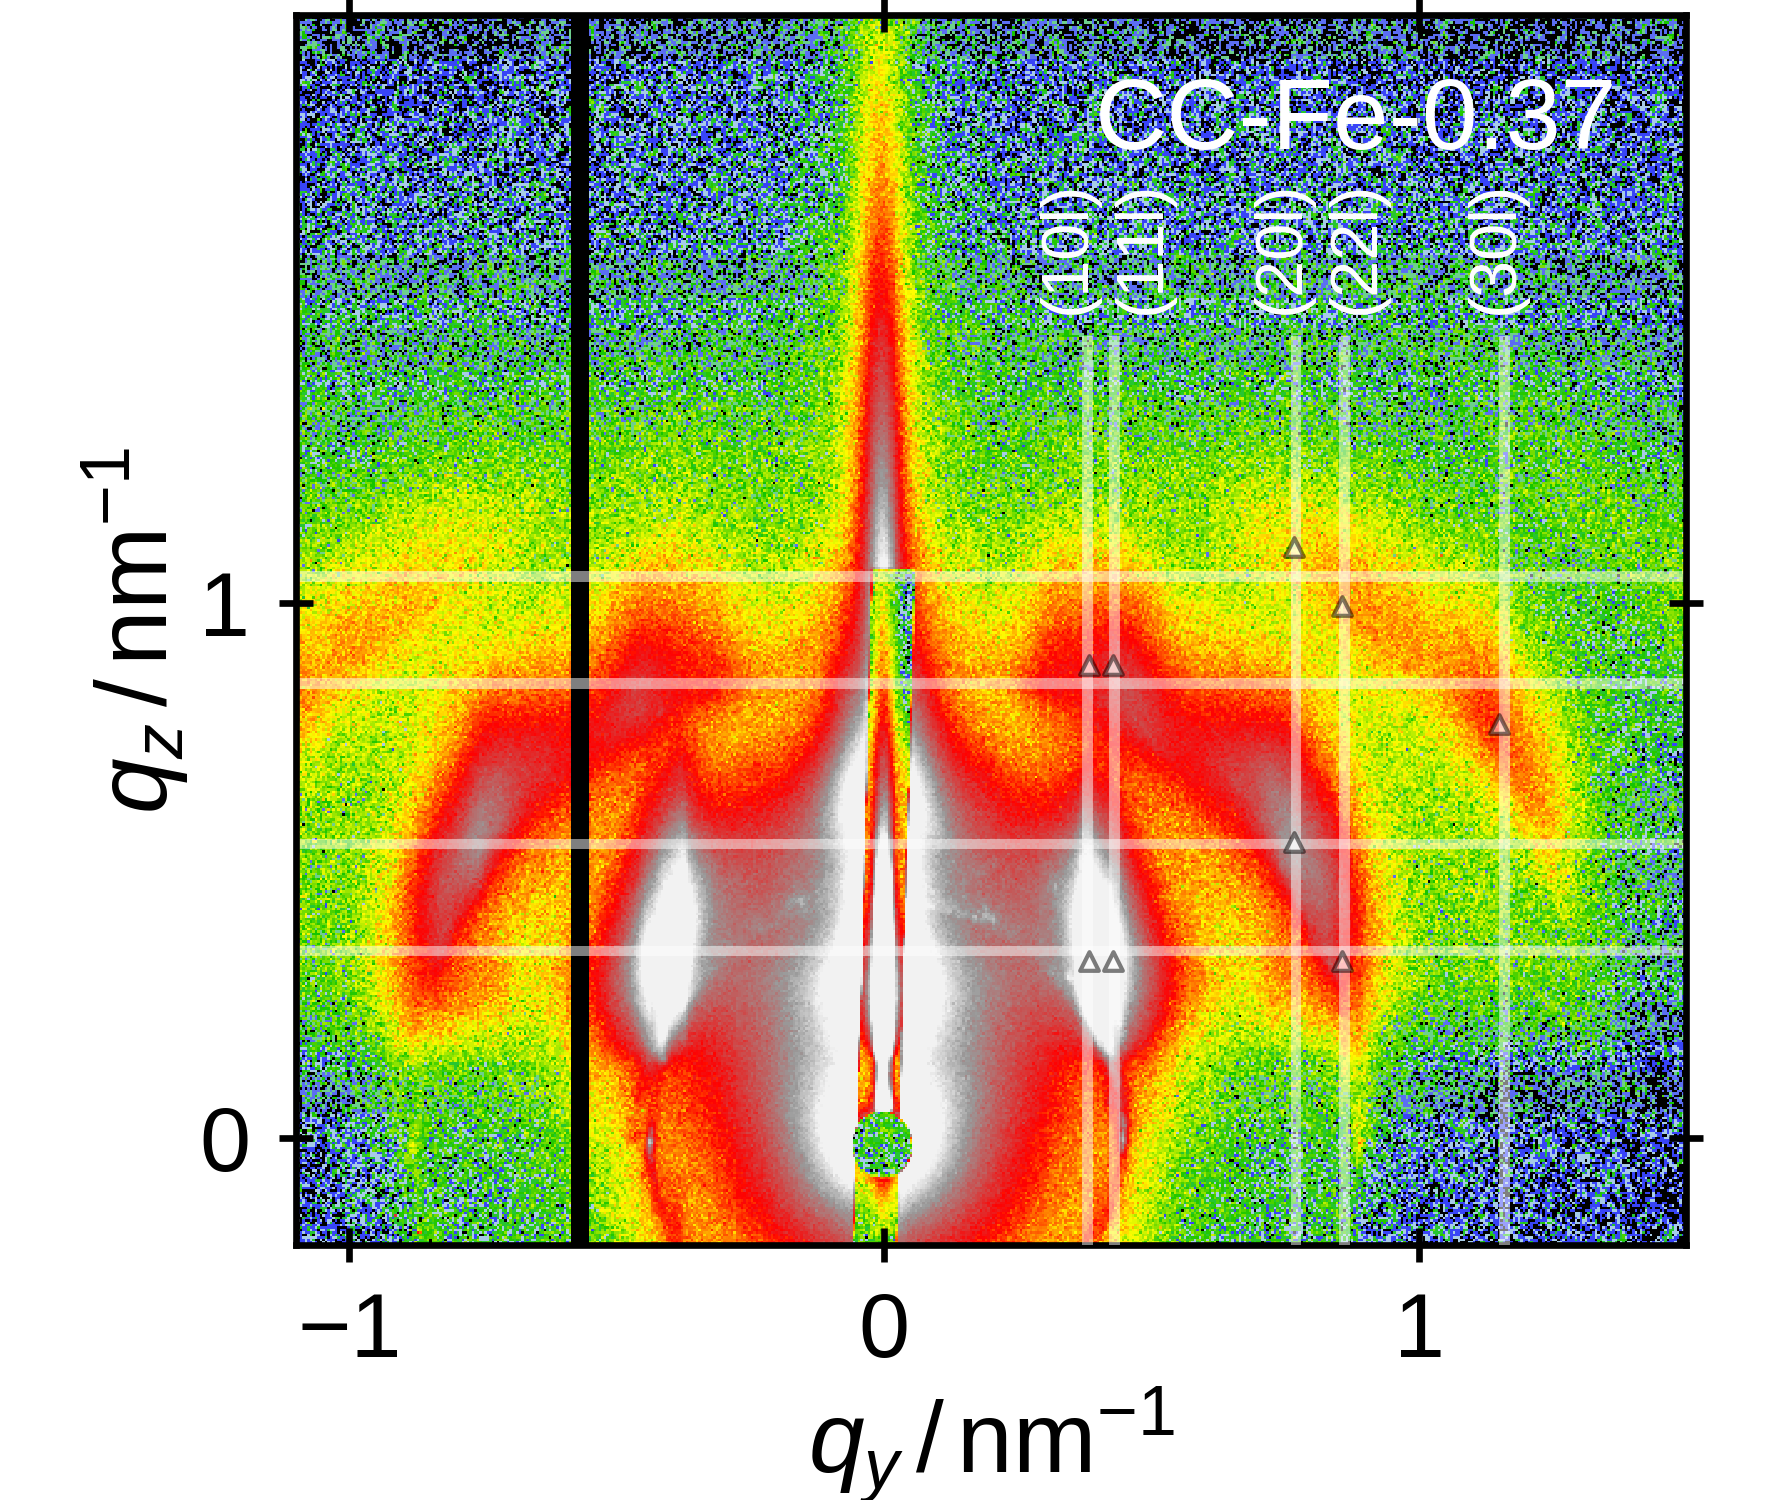
\includegraphics{colloidalCrystals_GISAXS_cut_CC-Fe-0_37}
    \caption{\label{fig:colloidalCrystals:layers:gisaxs}GISAXS data of CC-Fe-0.37 measured under an incident angle of $0.155 ^\circ$ (left) and $0.205 ^\circ$ (right). Additionally marked are the integrated areas for the cuts shown in \reffig{fig:colloidalCrystals:layers:gisaxsCuts}.}
  \end{figure}

  \begin{figure}[tb]
    \centering
    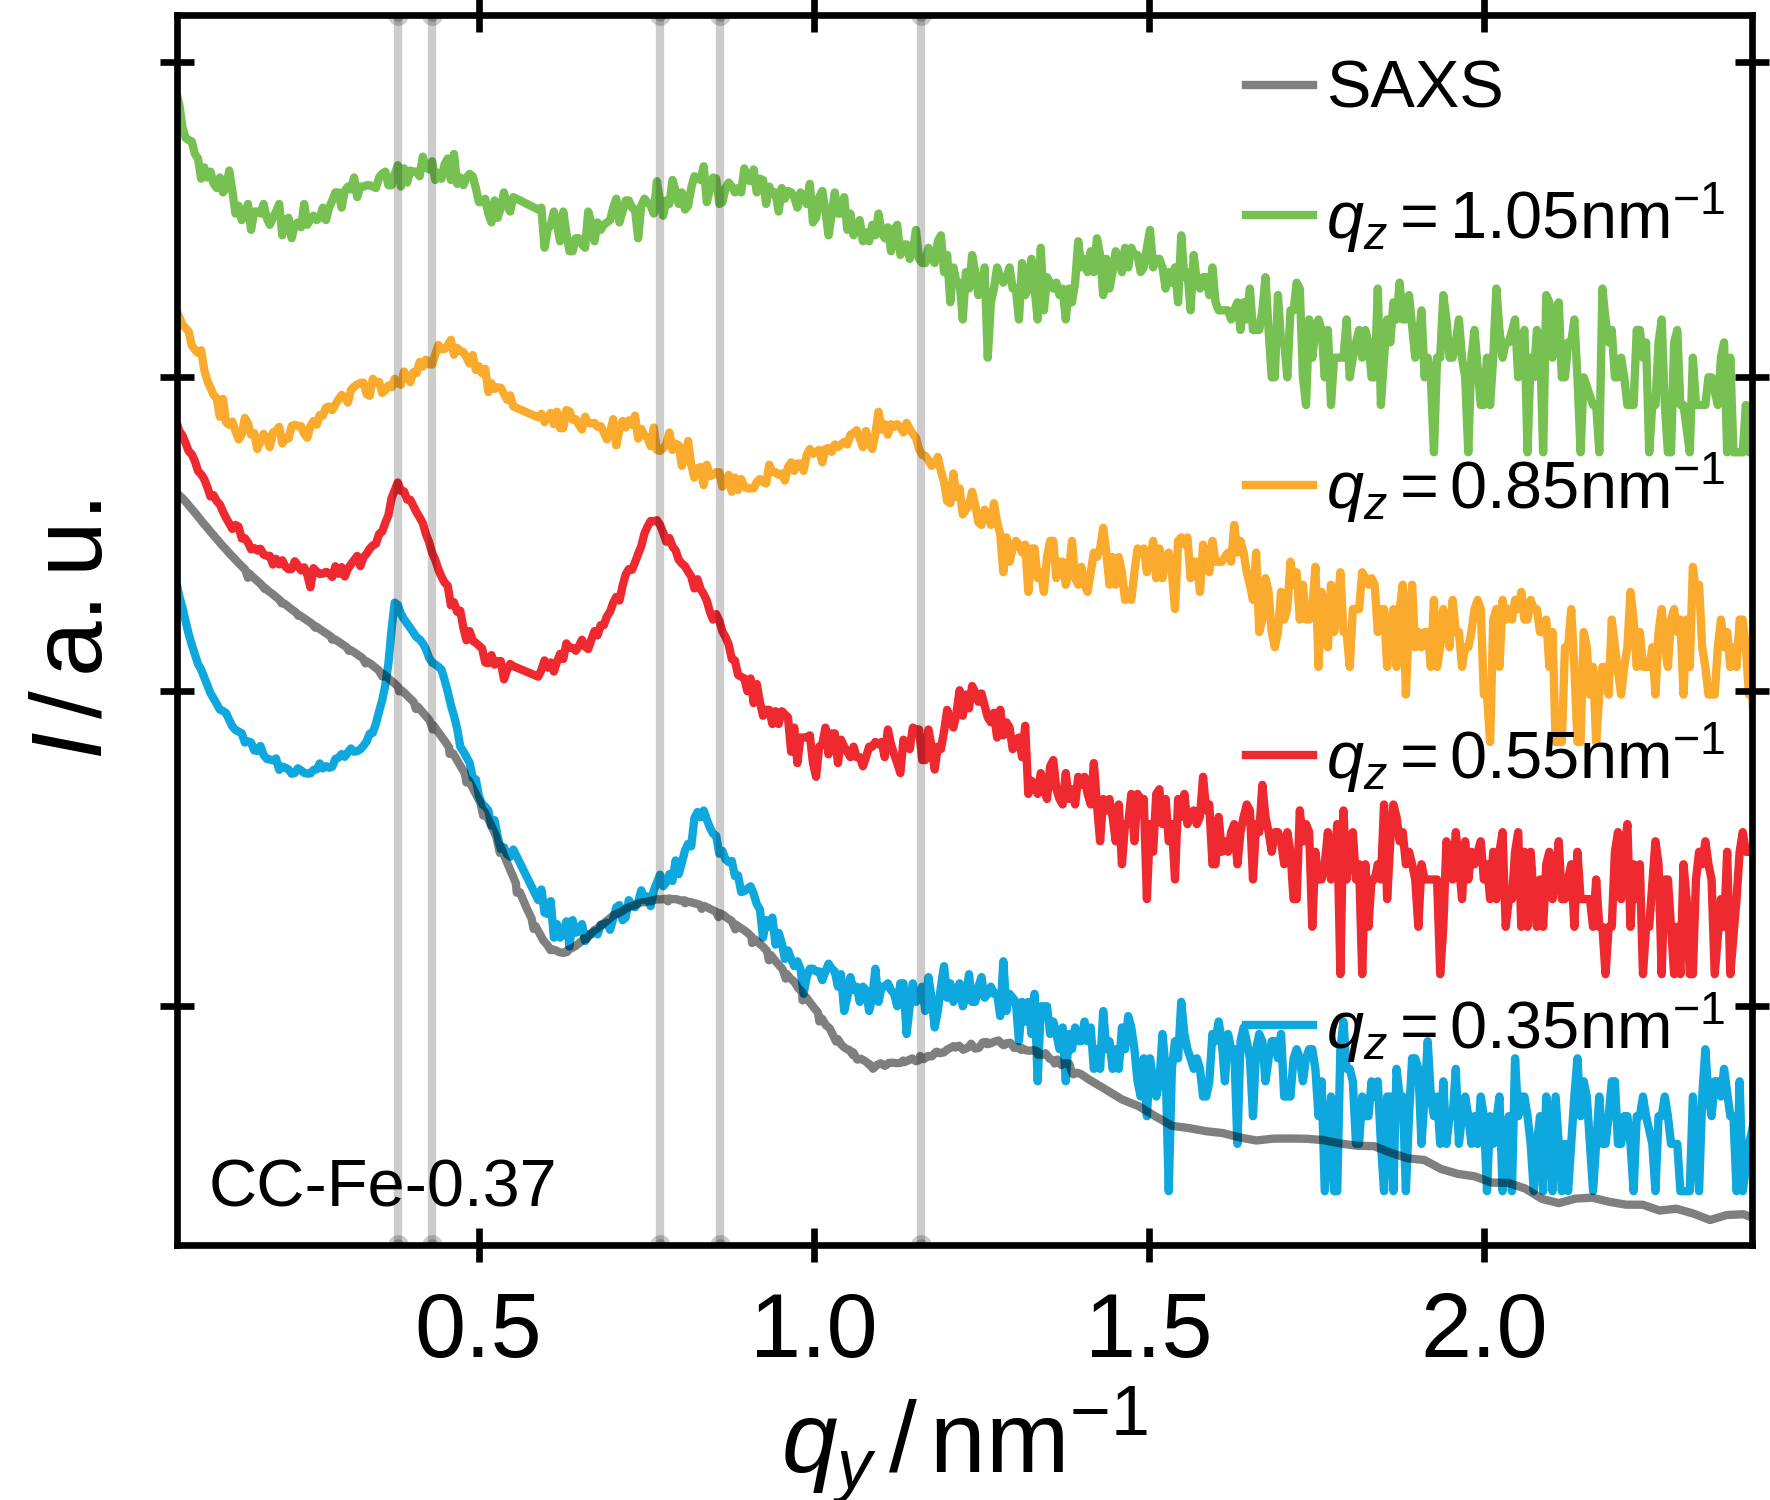
\includegraphics{colloidalCrystals_GISAXS_cut_horizontal_CC-Fe-0_37}
    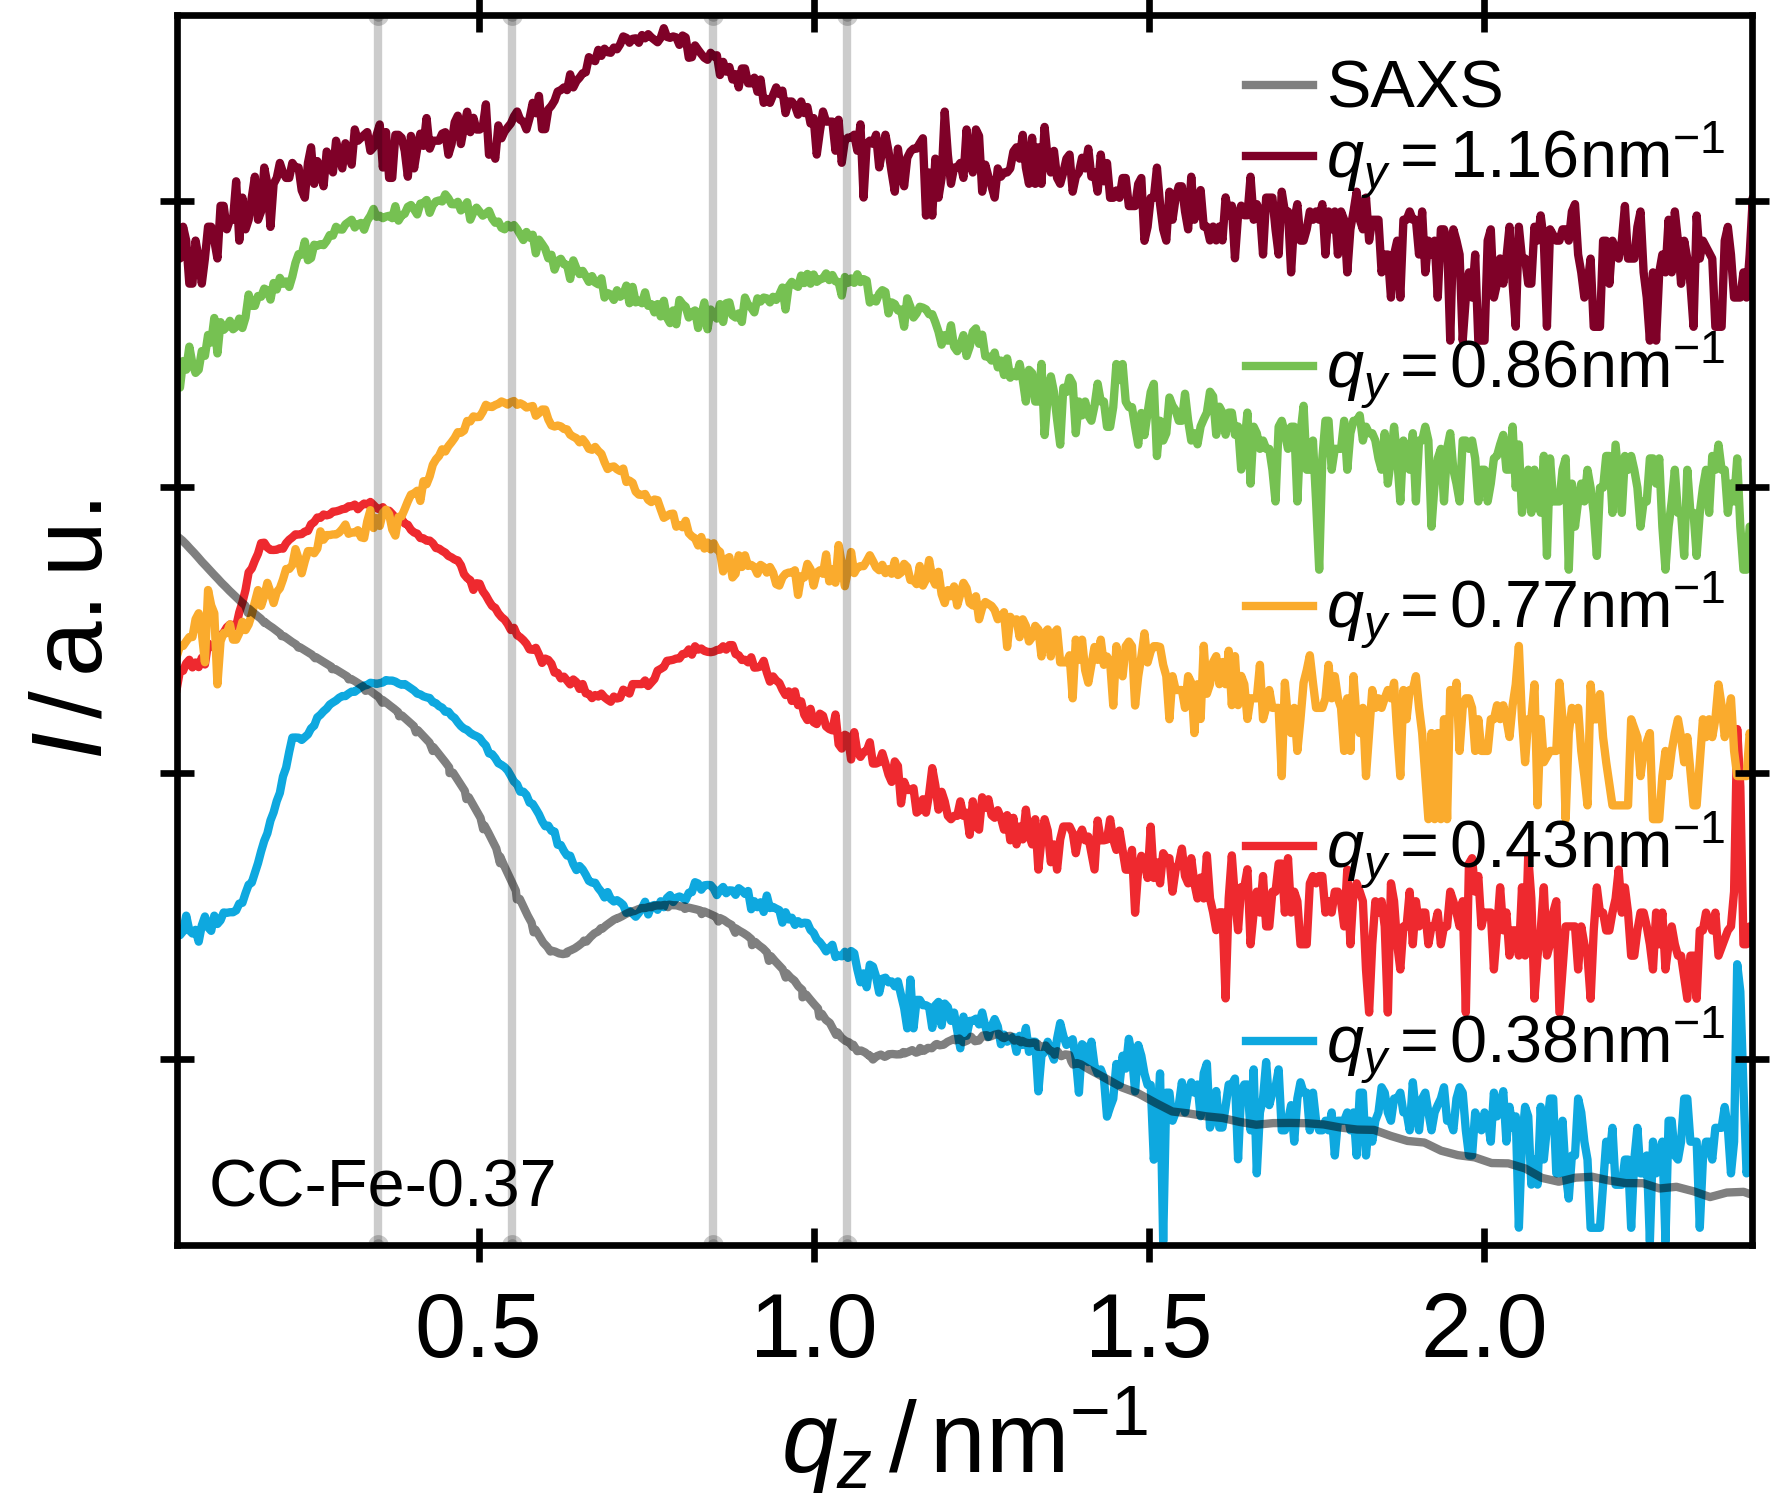
\includegraphics{colloidalCrystals_GISAXS_cut_vertical_CC-Fe-0_37}
    \caption{\label{fig:colloidalCrystals:layers:gisaxsCuts}Horizontal (left) and vertical (right) cuts in the GISAXS data of CC-Fe-0.37 shown in \reffig{fig:colloidalCrystals:layers:gisaxs}. For each line the data in a range of $\pm 0.01 \unit{nm^{-1}}$ around the given scattering vector is integrated.}
  \end{figure}


  % By suggestions of the cross-sectional SEM micrographs and following the structure evaluation of iron oxide mesocrystals in \cite{Wetterskog_2016_Tunin}, a body-centered tetragonal (bct) unit cell is used to index the observed peak positions.
  % Analogue to \cite{Wetterskog_2016_Tunin}, the tetragonal axes of the bct unit cell are set to a ratio of $c/a \eq \sqrt{3}$, and the indexing is performed with a [101]-orientation of the unit cell, which in a orthogonal lattice system has a rectangular unit cell with $b \eq 2a$ and $c \eq \sqrt{12} a$.

  To determine the superstructure of the nanocubes in the colloidal crystal, grazing-incidence small X-ray scattering is performed on the selected sample CC-Fe-0.37.
  The obtained detector images for the two incident angles $\alpha_i \eq 0.155^\circ$ and $\alpha_i \eq 0.205^\circ$ is shown in \reffig{fig:colloidalCrystals:layers:gisaxs}.
  The data shows the emergence of multiple broad peaks on top of additionally  weakly visible form factor rings.

  The broadness of the peaks and the elongation of the peak along $q_z$ alludes to the relatively thin layer structure of only few unit cells for the vertical direction in CC-Fe-0.37.
  Also the visibility of form factor rings can be interpret as a large fraction of nanocubes being randomly distributed.

  By performing multiple cuts, marked in the detector image and shown in \reffig{fig:colloidalCrystals:layers:gisaxsCuts}, the peak coordinates are determined.
  The peaks are indexed by a $bct$ unit cell with [101]-orientation.
  Setting $a \eq 16.4 \unit{nm}$ and $b \eq 2a$, the $q_y$ positions are identified to be indexed by $(10l)$, $(11l)$, $(20l)$, $(22l)$ and $(30l)$.
  Setting further $c \eq \sqrt{12} a$, visible peaks are identified for $l\eq 3,\, 8$ in the $(10l)$, $(11l)$ series, $l \eq 5, \, 10$ for $(20l)$, $l \eq 3,\, 9$ for $(22l)$ and $l\eq 10$ for $(30l)$.

  \begin{table}[!htbp]
    \centering
    \caption{\label{tab:colloidalCrystals:gisaxs:peaks}Determined peak positions from \reffig{fig:colloidalCrystals:layers:gisaxs} and their associated index in a $bct$ unit cell with [101]-orientation and lattice constants of $a \eq 16.4 \unit{nm}$, $b \eq 2a$ and $c \eq \sqrt{12}a$.}
    \begin{tabular}{ c | c | l }
      $q_y\,/ \unit{nm^{-1}}$ & $q_z\, / \unit{nm^{-1}}$ & index \\
      \hline
      $0.38$      & $0.35$  & (103)\\
      $0.38$      & $0.85$  & (108)\\
      $0.43$      & $0.35$  & (113)\\
      $0.43$      & $0.85$  & (118)\\
      $0.77$      & $0.55$  & (205)\\
      $0.77$      & $1.05$  & (2010)\\
      $0.86$      & $0.46$  & (223)\\
      $0.86$      & $1.05$  & (229)\\
      $1.16$      & $0.76$  & (3010)\\
      \hline
    \end{tabular}
  \end{table}

  Comparing the results to the mesocrystalline structure determined in literature \cite{Wetterskog_2016_Tunin} from drop casted iron oxide nanocubes with a similar size, to some degree the results are reproduced in this discussion.
  It's remarkable that the same $bct$ structure as in the study from drop casted nanoparticles is observed.
  With the only difference between the two methods being that one produces large towers of ordered nanocubes, and the other a connected layer.
  In the literature study, magnetic fields are further used during the drying process to manipulate the structure formation.
  Even though this should be an interesting case study also for this system, this is beyond the scope of this work and left for future studies.

\end{document}